\documentclass[11pt,a4paper]{article}
\usepackage[margin=27mm,headheight=15pt]{geometry}
\usepackage[T1]{fontenc}
\usepackage{amsmath,amsthm,mathtools}
\usepackage{newtxtext,newtxmath}
\usepackage{microtype}
\usepackage{graphicx,booktabs,array,tabularx}
\usepackage{xcolor,fancyhdr,enumitem,xurl}
\usepackage[hidelinks,pdftitle={Critical Complements in Fabius Conditioning},
 pdfauthor={Research manuscript prepared for Vladimir Reshetnikov}]{hyperref}
\definecolor{ink}{HTML}{203340}
\pagestyle{fancy}\fancyhf{}
\fancyhead[L]{\small Critical complements in Fabius conditioning}
\fancyhead[R]{\small Research manuscript}
\fancyfoot[C]{\thepage}
\setlength{\parskip}{3pt}
\setlength{\parindent}{1.2em}
\setlength{\emergencystretch}{2em}
\setcounter{tocdepth}{1}
\numberwithin{equation}{section}
\newtheorem{theorem}{Theorem}[section]
\newtheorem{lemma}[theorem]{Lemma}
\newtheorem{proposition}[theorem]{Proposition}
\newtheorem{corollary}[theorem]{Corollary}
\theoremstyle{definition}
\newtheorem{definition}[theorem]{Definition}
\newtheorem{question}{Question}
\theoremstyle{remark}
\newtheorem{remark}[theorem]{Remark}
\newcommand{\R}{\mathbb R}
\newcommand{\N}{\mathbb N}
\newcommand{\E}{\mathbb E}
\newcommand{\Pp}{\mathbb P}
\newcommand{\Var}{\operatorname{Var}}
\newcommand{\Cov}{\operatorname{Cov}}
\newcommand{\Law}{\mathcal L}
\newcommand{\Exp}{\operatorname{Exp}}
\newcommand{\TV}{d_{\mathrm{TV}}}
\newcommand{\KL}{D_{\mathrm{KL}}}
\newcommand{\ind}{\mathbf 1}
\newcommand{\eps}{\varepsilon}
\newcommand{\ov}{\mathcal O}
\newcommand{\HH}{\mathcal H}
\newcommand{\dd}{\mathrm d}
\newcommand{\repo}{\texttt{ProveIt}}
\newcommand{\snap}{\texttt{0a543d5e435df885f78ca731d71856f3ee0ab2d4}}
\newcommand{\gammak}[1]{\gamma_{#1}}
\DeclareMathOperator{\supp}{supp}

\makeatletter
\newcommand{\inputtable}[1]{\@@input#1 }
\makeatother

\begin{document}
\hypersetup{pageanchor=false}
\begin{titlepage}
\vspace*{7mm}
{\large\sffamily\color{ink} PROVEIT RESEARCH SERIES\par}
\vspace{13mm}
{\Huge\bfseries Critical Complements\par
in Fabius Conditioning\par}
\vspace{7mm}
{\Large Sharp information loss, geometric phase constants,\par
and a logarithmic crossover\par}
\vspace{10mm}
{\normalsize Prepared for Vladimir Reshetnikov\par
30 September 2026\par}
\vspace{11mm}
\begin{abstract}
Let $S_q=\sum_{j\ge1}q^jU_j$, with independent uniform coordinates and
$0<q<1$. Condition the original law on $S_q$ lying below its mean under a
large exponential tilt. The repository's earlier conditioning papers
identify when a coordinate block resembles its tilted product law, but
leave the critical-complement regime without sharp rates. We resolve its
geometric-prefix version: observe $n-m$ bulk coordinates, where $n$ is
the effective dimension and $m=o(n)$.

For fixed $m$, the overlap with the tilted product is
$[\tfrac12\log(2\pi n)+1+K_{q,\rho,m}]/\sqrt{2\pi n}
+o(n^{-1/2})$, with an explicit geometric-phase constant. Relative entropy
is $\tfrac12\log(2\pi n)-h(R_m+E)+O(n^{-1})$, and we calculate its
$1/n$ coefficient. An exact compact boundary correction explains the
slow convergence of the overlap expansion.

For $m\to\infty$, $m=o(n)$, relative entropy becomes
$\tfrac12\log(n/m)-\tfrac12+o(1)$. Total variation has a different,
three-regime structure. Its overlap crosses from $\log n/\sqrt n$ to
$\sqrt{(m/n)\log(n/m)}$ at $m\asymp\log n$. We give one leading formula
throughout, using the two real branches of Lambert $W$ and the Gamma
rate function. The information discarded by a fixed complement is
exactly an exponential-noise mutual information in the limit.

Proofs use an exact one-dimensional likelihood identity and a signed
Gamma-convolution calculus, not an unquantified Gaussian extrapolation.
The package includes reproducible floating-point diagnostics and a
further-research program.
\end{abstract}
\vfill
\noindent\small
\textbf{Status.} Conventional proofs in a research draft; not Lean-certified
or externally refereed. The resolved question is a specified repository
frontier, not a claimed solution of a named famous conjecture. Classical
Gibbs conditioning, log-concavity, and Gamma asymptotics are not claimed
as new. Worldwide priority has not been established.
\end{titlepage}
\hypersetup{pageanchor=true}
\pagenumbering{roman}
\tableofcontents
\clearpage
\pagenumbering{arabic}

\section{The question and its place in the repository}
\label{sec:context}

\subsection{From a qualitative endpoint to sharp asymptotics}
The probabilistic Fabius model is unusually well suited to studying rare
configurations. The event that a geometrically weighted sum of independent
uniform variables is very small constrains many coordinates simultaneously.
An exponential tilt removes most of the rarity, but conditioning on the
sum still couples the coordinates. The question is how much of that
coupling an observer can detect.

Two research manuscripts in the inspected \repo\ snapshot already address
this problem. \emph{Sharp Conditioning Laws for Uniform Random Series}
proves a variance-fraction criterion for general positive summable
weights, computes total-variation and entropy limits when the observed
variance fraction tends to a number strictly between zero and one, and
proves only the qualitative conclusions $\TV\to1$, $\KL\to\infty$ when
that fraction tends to one. Its further-research list and conclusion
explicitly leave critical complements and quantitative corrections open
\cite{repo-uniform}. A companion lacunary-series manuscript develops
full-configuration approximations, marginal corrections, fluctuation
processes, and boundary laws \cite{repo-lacunary}.

The present paper asks the following precise continuation question:
\begin{quote}
For geometric weights, how fast do the marginal total variation and
relative entropy approach their singular endpoints when the unobserved
bulk contains only $m=o(n)$ coordinates? What survives of the geometric
phase when $m$ stays bounded?
\end{quote}
The answer is not obtained by merely inserting a moving variance fraction
into a fixed-fraction limit. Relative entropy has a universal diverging
logarithm once $m\to\infty$, whereas overlap has a transition at
$m\asymp\log n$. Fixed complements retain a non-Gaussian boundary density
and explicit phase constants.

Our inspection is pinned to \snap. The relevant predecessor paths and
precise comparison are recorded in the bibliography and the package's
\texttt{provenance.json}. The repository is large; this is a targeted
comparison of the pertinent conditioning manuscripts, not an exhaustive
verification of every research report. The proofs below do not require
assuming the correctness of the unformalized predecessor theorems.

\subsection{Prior work and the contribution boundary}
Conditional approximation by exponential families is classical.
Diaconis and Freedman studied conditional limit theorems and finite
versions of de Finetti's theorem \cite{df}. Dembo and Zeitouni developed
refinements of the Gibbs conditioning principle, including growing blocks
\cite{dz}. Those works are the natural background for the small-block
question. The Fabius--Rvachev construction and its smooth compactly
supported density are described by Arias de Reyna \cite{arias}.

The contribution here is the proved critical-complement theorem package
for the moving geometric tilt: a fixed-complement phase expansion, a
uniform leading crossover for every $m=o(n)$, a sharp entropy constant,
and an information-loss interpretation. The Gamma rate function and
Lambert $W$ are standard tools. Nor is the general fact that a scalar
constraint becomes a likelihood depending on a block sum a new principle.
The value of the calculation is to identify the correct boundary profile,
to control its vanishing likelihood level, and to prove the change of
asymptotic regime with all normalizations specified.

There is no assertion here that a targeted literature search certifies
publication priority. The mathematical claims are the displayed theorems
and proofs. Their relationship to the entire conditional-limit literature
is a separate priority-review question.

\subsection{Conventions}
All logarithms are natural. For probability measures on the same space,
\[
\TV(P,Q)=\sup_A|P(A)-Q(A)|,\qquad
\KL(P\Vert Q)=\int\log\frac{\dd P}{\dd Q}\,\dd P.
\]
The overlap is $1-\TV(P,Q)=\int\min(\dd P,\dd Q)$; there is no extra factor
of two in this definition. Differential entropy is
$h(g)=-\int g\log g$, with $0\log0=0$. All big-$O$ constants may depend on
fixed $q$ and $\rho$. A fixed-$m$ statement permits dependence on $m$ as
well; it is not uniform in a growing complement unless explicitly stated.

\section{Model and main results}
\label{sec:results}

\subsection{The phase convention and the observed block}
Let
\begin{equation}\label{eq:series}
S_q=\sum_{j\ge1}q^jU_j,\qquad
U_j\overset{\mathrm{iid}}\sim\operatorname{Unif}[0,1],\qquad 0<q<1.
\end{equation}
Write $P$ for the original product law. Fix $1\le\rho<q^{-1}$ and put
\begin{equation}\label{eq:tilt}
t_n=\rho q^{-(n+1)},\quad T_n=t_nS_q,\quad
\frac{\dd Q_n}{\dd P}=\frac{e^{-T_n}}{\E_P e^{-T_n}},\quad
\mu_n=\E_{Q_n}T_n,\quad x_n=\mu_n/t_n.
\end{equation}
Our conditioned law is
\begin{equation}\label{eq:condition}
P_n=P(\,\cdot\mid S_q\le x_n).
\end{equation}
The boundary starts at coordinate $n+1$, whose scaled cap is $\rho$.
We call the first $n$ coordinates the bulk. This is a phase convention,
not a claim that the physical transition consists of an abrupt cutoff.

Under $Q_n$, the variables $X_{n,j}=t_nq^jU_j$ are independent, with
\begin{equation}\label{eq:te}
p_a(x)=\frac{e^{-x}}{1-e^{-a}}\ind_{(0,a)}(x),\qquad
 a=t_nq^j.
\end{equation}
For $0\le m<n$, observe the prefix $B_{n,m}=\{1,\ldots,n-m\}$.
Let $P_{n,m}$ and $Q_{n,m}$ be the corresponding marginals of $P_n$ and
$Q_n$, and set
\[
\ov_{n,m}=1-\TV(P_{n,m},Q_{n,m}),\qquad
D_{n,m}=\KL(P_{n,m}\Vert Q_{n,m}),\qquad
\eps_n=(2\pi n)^{-1/2}.
\]
The complement contains $m$ bulk coordinates \emph{and the whole infinite
boundary tail}. In particular, $m=0$ does not mean observing the entire
infinite configuration.

\subsection{The exact complement object}
On a separate product space, let the $Y_\ell$ be independent with density
$p_{\rho q^\ell}$, and define
\begin{equation}\label{eq:Rm}
R_m=\sum_{\ell=-m}^{\infty}Y_\ell,\quad
r_m=\E R_m,\quad Z_m=R_m+E,\quad E\sim\Exp(1)
\end{equation}
with $E$ independent of the series. The complement under $Q_n$ has exactly
the law of $R_m$, not just an asymptotic approximation. Write $g_m$ for
the density of $Z_m$ and $h_m=h(g_m)$. Further set
\begin{equation}\label{eq:AK}
A_m=\frac{\rho q^{-m}}{1-q},\qquad
K_m=K_{q,\rho,m}=\log\E e^{R_m}
 =\sum_{\ell=-m}^{\infty}
   \log\frac{\rho q^\ell}{1-e^{-\rho q^\ell}}.
\end{equation}
Thus $0\le R_m\le A_m$. All these quantities are finite for fixed $m$.
The extra exponential variable in $Z_m$ is essential: it arises from the
inequality in \eqref{eq:condition}.

For later refinements define
\begin{align}
v(a)&=1-\frac{a^2e^a}{(e^a-1)^2},\label{eq:varone}\\
\delta&=\sum_{r=1}^{\infty}\{v(\rho q^{-r})-1\}
          +\sum_{\ell=0}^{\infty}v(\rho q^\ell),\label{eq:delta}\\
\mathscr E_m&=\frac{\delta}{2}+\frac1{12}
 -\frac12\Cov\!\left((Z_m-\E Z_m)^2,\log g_m(Z_m)\right).
\label{eq:Ecoeff}
\end{align}
Here $v(a)$ is the variance of $p_a$. The series defining $\delta$ converges;
indeed $\Var_{Q_n}(T_n)=n+\delta+o(1)$.

\subsection{Fixed complements: phase constants and a quantitative correction}
\begin{theorem}[Fixed-complement expansion]\label{thm:fixed}
For fixed $q,\rho,m$, as $n\to\infty$,
\begin{align}
\ov_{n,m}
 &=\eps_n\left(\log\frac1{\eps_n}+1+K_m\right)+o(\eps_n),
 \label{eq:fixedtv}\\
D_{n,m}
 &=\log\frac1{\eps_n}-h_m+\frac{\mathscr E_m}{n}+O(n^{-2}).
 \label{eq:fixedkl}
\end{align}
More precisely, with
\begin{equation}\label{eq:deficit}
\Delta_m(a)=\int_0^{A_m}\left(1-\frac{g_m(u)}a\right)_+\,\dd u,
\end{equation}
one has $\Delta_m(a)\to0$ as $a\downarrow0$ and
\begin{equation}\label{eq:correctedtv}
\ov_{n,m}=\eps_n\left(\log\frac1{\eps_n}+1+K_m-
                  \Delta_m(\eps_n)\right)
       +O\!\left(\frac{\eps_n(\log n)^3}{n}\right).
\end{equation}
\end{theorem}
The compact integral $\Delta_m$ is an exact profile correction, not a
fitted coefficient. For the dyadic example it explains why convergence
to \eqref{eq:fixedtv} is visibly much slower than convergence of entropy.
The proof is in Section~\ref{sec:fixed}.

\subsection{Every sublinear complement: the overlap crossover}
Let $I(y)=y-1-\log y$ for $y>0$. For $z>0$, denote the two solutions of
$I(y)=z$ by
\begin{equation}\label{eq:roots}
y_-(z)=-W_0(-e^{-1-z})<1,
\qquad y_+(z)=-W_{-1}(-e^{-1-z})>1.
\end{equation}
\begin{theorem}[Critical-complement crossover]\label{thm:crossover}
Let $1\le m=m_n<n$ and $m=o(n)$. Put
$d_{n,m}=\tfrac12\log(n/m)$ and $z_{n,m}=d_{n,m}/m$. Then
\begin{equation}\label{eq:unified}
\ov_{n,m}\sim\frac{m}{\sqrt{2\pi n}}
   \bigl[y_+(z_{n,m})-y_-(z_{n,m})\bigr].
\end{equation}
In particular,
\begin{align}
m=o(\log n):\quad
&\ov_{n,m}\sim\frac{\log n}{2\sqrt{2\pi n}},
\label{eq:thin}\\
\frac m{\log n}\to c\in(0,\infty):\quad
&\ov_{n,m}\sim\frac{\log n}{\sqrt{2\pi n}}C(c),\qquad
 C(c)=c\bigl[y_+(1/(2c))-y_-(1/(2c))\bigr],
\label{eq:critical}\\
\log n=o(m),\quad m=o(n):\quad
&\ov_{n,m}\sim\sqrt{\frac2\pi}\,
        \sqrt{\frac mn\log\frac nm}.
\label{eq:gaussian}
\end{align}
The first assertion \eqref{eq:thin} also holds for $m=0$ and for sequences
that take the value zero. Moreover,
\begin{equation}\label{eq:Cends}
C(c)\longrightarrow\frac12\quad(c\downarrow0),\qquad
C(c)\sim2\sqrt c\quad(c\to\infty).
\end{equation}
\end{theorem}
Equation~\eqref{eq:unified} is a leading equivalent, not a second-order
expansion. In particular, expanding its Lambert roots further at fixed
$m$ does not replace the phase expansion in Theorem~\ref{thm:fixed}.

All three regimes have $\TV\to1$. What changes is the small amount of
mass that the two laws still share. Section~\ref{sec:crossover} proves
\eqref{eq:unified} by treating the possible limits of $z_{n,m}$; no
unproved uniform substitution into a fixed-fraction theorem is used.

\subsection{Entropy and information loss}
\begin{theorem}[Entropy with a growing critical complement]\label{thm:entropy}
If $m\to\infty$ and $m=o(n)$, then
\begin{equation}\label{eq:growingkl}
D_{n,m}=\frac12\log\frac nm-\frac12+o(1).
\end{equation}
For the entire infinite configuration,
\begin{equation}\label{eq:fullkl}
\KL(P_n\Vert Q_n)=\frac12\log(2\pi n)-1+o(1).
\end{equation}
Consequently, for each fixed $m$,
\begin{equation}\label{eq:infogap}
\KL(P_n\Vert Q_n)-D_{n,m}
 \longrightarrow h(R_m+E)-1=I(R_m;R_m+E).
\end{equation}
\end{theorem}
The mutual information on the right is finite and strictly positive.
Its interpretation is precise: the limiting cost of hiding the boundary
complement is the information that its tilted sum transmits through
independent one-sided exponential noise. The proof is in
Section~\ref{sec:entropy}.

\section{An exact likelihood and the Fabius boundary profile}
\label{sec:likelihood}

\subsection{Existence of the tilted product}
The original series converges absolutely, since
$0\le S_q\le q/(1-q)$. Its Laplace transform is positive. Finite product
factorization and bounded convergence therefore give the tilted product
in \eqref{eq:te}, including independence of any finite coordinate set
from its infinite tail. The mean and variance of one coordinate are
\begin{equation}\label{eq:moments}
b(a)=1-\frac a{e^a-1},\qquad
v(a)=1-\frac{a^2e^a}{(e^a-1)^2}.
\end{equation}
They follow by differentiating the integral of $e^{-x}$ over $(0,a)$.
At zero, $b(a)=a/2+O(a^2)$ and $v(a)=a^2/12+O(a^4)$; at infinity,
$b(a)=1+O(ae^{-a})$ and $v(a)=1+O(a^2e^{-a})$.
It follows that
\begin{equation}\label{eq:meanvar}
\mu_n=n+c_{q,\rho}+o(1),\qquad
\Var_{Q_n}(T_n)=n+\delta+o(1),
\end{equation}
where
\[
c_{q,\rho}=r_0-\sum_{r\ge1}\frac{\rho q^{-r}}{e^{\rho q^{-r}}-1}.
\]
The errors in \eqref{eq:meanvar} in fact decrease faster than any inverse
power of $n$. Also $r_m=m+O(1)$ and $\Var(R_m)=m+O(1)$, uniformly in $m$.

\subsection{The density that controls the answer}
\begin{proposition}[Exact boundary profile]\label{prop:profile}
Let $F_q(x)=P(S_q\le x)$, extended by zero and one outside its support.
For $u>0$,
\begin{equation}\label{eq:gprofile}
g_m(u)=e^{-u}\E\bigl[e^{R_m}\ind_{\{R_m\le u\}}\bigr]
      =e^{K_m-u}F_q\!\left(\frac{q^{m+1}u}{\rho}\right).
\end{equation}
The density is continuous, positive on $(0,\infty)$, log-concave, bounded
by one, and satisfies the exact tail identity
\begin{equation}\label{eq:tail}
g_m(u)=e^{K_m-u}\quad\text{for }u\ge A_m.
\end{equation}
Its entropy and all integrals
$\int(1+u^j)g_m(u)|\log g_m(u)|\,\dd u$, $j\ge0$, are finite.
\end{proposition}
\begin{proof}
Convolution with the independent $E$ gives the first equality in
\eqref{eq:gprofile}. Before tilting, the complement sum has the law of
$\rho q^{-m-1}S_q$. Its tilted law is obtained by multiplying by $e^{-u}$
and normalizing. Since the support is bounded, reversing this tilt
inside the expectation is legitimate and gives the second equality.
The normalization is $\E e^{R_m}=e^{K_m}$, obtained by taking the product
of the one-coordinate integrals $a/(1-e^{-a})$.

Every positive interval $(0,u)$ has positive complement probability:
choose a finite prefix small enough and make its deterministic remaining
tail less than $u/2$. This also shows $F_q(x)>0$ for $x>0$. The complement
has no atoms because one of its independent summands has a density.
Continuity of its CDF gives continuity of $g_m$. The first expression in
\eqref{eq:gprofile} gives $g_m\le1$ directly. The tail identity follows
from $R_m\le A_m$.

Each truncated exponential density, and the exponential density, is
log-concave. Convolution preserves log-concavity by Pr\'ekopa's theorem
\cite[Theorem~7]{prekopa}. Apply that result to finite partial sums plus
$E$. Their densities converge pointwise to $g_m$: in the first formula
of \eqref{eq:gprofile}, partial sums converge almost surely, the
exponential factor is bounded for fixed $m$, and the limiting sum has
no atoms. Pointwise limits preserve the log-concavity inequality.
Finally, $-x\log x$ is bounded on $[0,1]$, so the entropy integrand is
integrable on $[0,A_m]$. The exact exponential tail handles every
polynomially weighted integral on the remainder of the half-line.
\end{proof}

\subsection{Reduction of both distances to one dimension}
Let
\[
W_{n,m}=\sum_{j\in B_{n,m}}X_{n,j},\qquad
V_{n,m}=W_{n,m}-\E_{Q_n}W_{n,m},
\]
and let $f_{n,m}$ denote the density of the centered sum $V_{n,m}$.
Extend this density by zero off its support. Define the common
normalizer
\begin{equation}\label{eq:an}
a_n=\E_{Q_n}\bigl[e^{T_n-\mu_n}\ind_{\{T_n\le\mu_n\}}\bigr].
\end{equation}
It depends on $n,q,\rho$, but not on the chosen prefix.

\begin{proposition}[Exact marginal likelihood]\label{prop:likelihood}
The likelihood of the conditioned prefix relative to its tilted product
law is
\begin{equation}\label{eq:likelihood}
\frac{\dd P_{n,m}}{\dd Q_{n,m}}
 =\frac{g_m(r_m-V_{n,m})}{a_n}.
\end{equation}
Under $P_{n,m}$, the variable $u=r_m-V_{n,m}$ has density
\begin{equation}\label{eq:udensity}
p^*_{n,m}(u)=\frac{f_{n,m}(r_m-u)g_m(u)}{a_n},\quad u>0.
\end{equation}
In particular,
\begin{align}
a_n&=\int_0^\infty f_{n,m}(r_m-u)g_m(u)\,\dd u,
\label{eq:aintegral}\\
\ov_{n,m}&=\int_0^\infty f_{n,m}(r_m-u)
                  \min\{1,g_m(u)/a_n\}\,\dd u,
\label{eq:overlapexact}\\
D_{n,m}&=-\log a_n+
 \int_0^\infty p^*_{n,m}(u)\log g_m(u)\,\dd u.
\label{eq:entropyexact}
\end{align}
\end{proposition}
\begin{proof}
Changing from $P$ to $Q_n$ in the conditioning event gives the full
likelihood $e^{T_n-\mu_n}\ind_{\{T_n\le\mu_n\}}/a_n$.
Given a prefix with centered sum $v$, the independent complement is $R_m$
and $T_n-\mu_n=v+R_m-r_m$. Conditional expectation of the full likelihood
is therefore
\[
\frac{e^{v-r_m}}{a_n}
  \E\bigl[e^{R_m}\ind_{\{R_m\le r_m-v\}}\bigr]
 =\frac{g_m(r_m-v)}{a_n}.
\]
This proves \eqref{eq:likelihood}. A change of variable from $v$ to
$u=r_m-v$ proves \eqref{eq:udensity} and its normalization. Integrating
$\min(1,\dd P_{n,m}/\dd Q_{n,m})$ gives the overlap. Integrating the
logarithm of the likelihood under $P_{n,m}$ gives the entropy formula.
All formulas concern the entire prefix marginal, not merely an
approximation by its sum: the likelihood is exactly a function of that sum.
\end{proof}

\begin{remark}[Why inequality conditioning matters]
For a regular conditional law on an exact level $T_n=\mu_n$, the analogous
complement factor is the density of $R_m$, not that of $R_m+E$. The
exponential tail \eqref{eq:tail}, the constant $1$ in the overlap, and
the information gap \eqref{eq:infogap} all use the inequality in the
present problem. Interchanging these two conditioning operations would
change the answer.
\end{remark}

\section{Signed Gamma convolutions and local estimates}
\label{sec:gamma}

\subsection{An exact algebraic representation}
Write
\[
\gamma_k(x)=\frac{e^{-x}x^{k-1}}{\Gamma(k)}\ind_{(0,\infty)}(x)
\]
for the unit-rate Gamma density. Put $a_r=\rho q^{-r}$ for $r\ge1$ and
introduce the finite signed measure
\begin{equation}\label{eq:nua}
\nu_a=\frac{\delta_0-e^{-a}\delta_a}{1-e^{-a}}.
\end{equation}
The elementary identity
\begin{equation}\label{eq:singleconv}
p_a=\gamma_1*\nu_a
\end{equation}
is valid pointwise away from endpoints. Although $\nu_a$ is signed,
the convolution on the right is the nonnegative truncated exponential
density. For $k=n-m$,
\begin{equation}\label{eq:prefixgamma}
\Law(W_{n,m})\text{ has density }
 \gamma_k*\nu_{m,n},\qquad
 \nu_{m,n}=\nu_{a_{m+1}}*\cdots*\nu_{a_n}.
\end{equation}
This is an exact identity for the actual geometric model.

\begin{lemma}[Uniform control of the signed correction]\label{lem:signed}
For every $0\le\theta<1$ there is a finite $C_\theta$, depending only on
$q,\rho,\theta$, such that
\begin{equation}\label{eq:weightedtv}
\int e^{\theta u}\,|\nu_{m,n}|(\dd u)\le C_\theta
       \quad(0\le m<n).
\end{equation}
Every $\nu_{m,n}$ has total mass one and support in $[0,\infty)$.
For fixed $m$ it converges in these weighted total-variation norms to
$\nu_{m,\infty}$. The error decreases faster than any inverse power
of $n$. Also $\nu_{m,\infty}\to\delta_0$ in the same norms as $m\to\infty$.
\end{lemma}
\begin{proof}
The weighted variation of a convolution is at most the product of the
weighted variations. Hence the left side of \eqref{eq:weightedtv} is at
most
\[
\prod_{r=m+1}^n
\frac{1+e^{-(1-\theta)a_r}}{1-e^{-a_r}}
\le\prod_{r=1}^{\infty}
\frac{1+e^{-(1-\theta)a_r}}{1-e^{-a_r}}<\infty.
\]
Convergence follows because $a_r$ grows geometrically and
$\sum_r e^{-c a_r}<\infty$ for every $c>0$. More explicitly,
$\nu_a-\delta_0=e^{-a}(\delta_0-\delta_a)/(1-e^{-a})$.
Telescoping the convolution product bounds the tail norm by a constant
multiple of $\sum_{r>N}e^{-(1-\theta)a_r}$. This proves all convergence
claims, including the stated speed. Mass and support follow directly
from \eqref{eq:nua}.
\end{proof}
The signed representation is only an analytic device. No probabilistic
argument treats a signed measure as the law of a random variable.

\subsection{Central density estimates and their first correction}
Define
\begin{equation}\label{eq:dm}
d_m=\sum_{r=m+1}^{\infty}\{v(a_r)-1\},\qquad
B_m(v)=\frac m2-\frac{v^2}{2}-v-\frac{d_m}{2}-\frac1{12}.
\end{equation}
\begin{lemma}[Prefix density estimates]\label{lem:local}
Suppose $m=o(n)$. Then
\begin{equation}\label{eq:globalf}
\sup_v f_{n,m}(v)\le C\eps_n,
\end{equation}
and for every sequence $b_n=o(\sqrt n)$,
\begin{equation}\label{eq:flatf}
\sup_{|v|\le b_n}\left|\frac{f_{n,m}(v)}{\eps_n}-1\right|\longrightarrow0.
\end{equation}
If $m$ is fixed, then for every fixed $C_0$, uniformly for
$|v|\le C_0\log n$,
\begin{equation}\label{eq:firstf}
f_{n,m}(v)=\eps_n\left[1+\frac{B_m(v)}n
                +O\!\left(\frac{1+|v|^6}{n^2}\right)\right].
\end{equation}
\end{lemma}
\begin{proof}
Stirling's formula gives $\sup_x\gamma_k(x)\le C/\sqrt k$. Combine it
with \eqref{eq:prefixgamma} and \eqref{eq:weightedtv} to obtain
\eqref{eq:globalf}. The mean shift of the signed correction is
\[
\beta_{m,n}=\int u\,\nu_{m,n}(\dd u)
 =-\sum_{r=m+1}^n\frac{a_r}{e^{a_r}-1},
\]
which is bounded uniformly. Thus
\[
f_{n,m}(v)=\int\gamma_k(k+\beta_{m,n}+v-u)\,\nu_{m,n}(\dd u).
\]
For $|w|=o(\sqrt k)$, uniformly,
$\sqrt{2\pi k}\,\gamma_k(k+w)\to1$. Restrict the signed integral to
$u\le h_n$, where $h_n\to\infty$ and $h_n=o(\sqrt n)$, and use the
exponential variation bound on the rest. Its signed mass is one. Since
$k/n\to1$, this proves \eqref{eq:flatf}.

For the refinement, Stirling's formula and the Taylor expansion of
$\log(1+w/k)$ give, uniformly on logarithmic windows,
\begin{equation}\label{eq:gammacentral}
\gamma_k(k+w)=\frac1{\sqrt{2\pi k}}
 \left[1-\frac{w^2/2+w+1/12}{k}
       +O\!\left(\frac{1+|w|^6}{k^2}\right)\right].
\end{equation}
Integrate this expansion against the signed correction. To justify the
integration of the remainder, first restrict to $u\le C_1\log n$ with
$C_1$ sufficiently large. The excluded weighted variation is smaller
than any prescribed inverse power of $n$, by \eqref{eq:weightedtv}; all
remaining polynomial moments are uniformly bounded. The first two
signed centered moments are zero and
$\Var(W_{n,m})-k=d_m+o(n^{-N})$ for every fixed $N$.
Consequently, after centering,
\[
\int w\,\dd\nu_{m,n}=v,\qquad
\int w^2\,\dd\nu_{m,n}=v^2+d_m+o(n^{-N}).
\]
Finally $(2\pi k)^{-1/2}=\eps_n[1+m/(2n)+O(n^{-2})]$.
Substitution in \eqref{eq:gammacentral} proves \eqref{eq:firstf}.
\end{proof}

\begin{corollary}[Normalization to two orders]\label{cor:normalizer}
With $\delta$ from \eqref{eq:delta},
\begin{equation}\label{eq:normalizerexp}
a_n=\eps_n\left[1-\frac{\delta/2+1/12}{n}+O(n^{-2})\right].
\end{equation}
In particular $a_n/\eps_n\to1$.
\end{corollary}
\begin{proof}
Use \eqref{eq:aintegral} with $m=0$ and apply
\eqref{eq:firstf}. The exponential tail of $g_0$ permits restriction
to $u\le C\log n$ with an error of arbitrarily high inverse-polynomial
order, using the global bound on $f$. All required polynomial moments
are finite. More generally, for any fixed $m$, if $Z_m$ has density
$g_m$, then
\[
\E(r_m-Z_m)=-1,\quad
\E(r_m-Z_m)^2=\Var(R_m)+2,
\]
so
\begin{equation}\label{eq:meanB}
\E B_m(r_m-Z_m)=-\frac\delta2-\frac1{12},
\end{equation}
because $d_m+\Var(R_m)-m=\delta$. Integrating the polynomial remainder
in \eqref{eq:firstf} gives $O(n^{-2})$.
\end{proof}

\subsection{A uniform saddle estimate for the complement}
Put
\begin{equation}\label{eq:Hdef}
\HH_m(s)=\E e^{sR_0}\prod_{r=1}^m
 \frac{1-e^{-(1-s)a_r}}{1-e^{-a_r}},\qquad \Re s<1.
\end{equation}
The product converges locally uniformly, together with all derivatives,
to an analytic function $\HH(s)$. It is strictly positive for real $s<1$
and $\HH(0)=1$. Directly from the truncated exponential integrals,
\begin{equation}\label{eq:mgf}
\E e^{sZ_m}=(1-s)^{-(m+1)}\HH_m(s),\qquad \Re s<1.
\end{equation}

\begin{lemma}[Complement saddle estimate]\label{lem:saddle}
For any compact interval $J\subset(0,\infty)$, uniformly for $y\in J$,
\begin{equation}\label{eq:saddle}
g_m(my)=\frac{\HH(1-1/y)}{\sqrt{2\pi m}}
          e^{-mI(y)}\,[1+O_J(m^{-1})],\qquad m\to\infty.
\end{equation}
Also, uniformly for $y$ in a compact interval on either side of one,
\begin{align}
\Pp(Z_m\ge my)&\le C_J e^{-mI(y)}&& (y>1),\label{eq:chernoffup}\\
\Pp(Z_m\le my)&\le C_J e^{-mI(y)}&& (y<1).
\label{eq:chernoffdown}
\end{align}
The constants in these tail bounds remain bounded as $y\to1$.
\end{lemma}
\begin{proof}
Let $\eta_m=\Law(R_0)*\nu_{0,m}$. The signed convolution identity gives
\begin{equation}\label{eq:gammacomplement}
g_m=\gamma_{m+1}*\eta_m.
\end{equation}
The measures $\eta_m$ have support in $[0,\infty)$, mass one, and
uniformly bounded exponentially weighted variations for every exponent
less than one. Their moment generating functions are $\HH_m$.
For $u\ge0$,
\begin{equation}\label{eq:gammaratio}
\frac{\gamma_{m+1}(my-u)}{\gamma_{m+1}(my)}
 =e^u\left(1-\frac{u}{my}\right)^m\ind_{\{u<my\}}.
\end{equation}
If $s=1-1/y$, this converges to $e^{su}$. Moreover,
$\log(1-z)\le-z$ bounds the ratio by $e^{su}$. Choose $\theta<1$
strictly larger than every $s$ arising from $J$. The exponential
variation bound makes the integration uniform in $y$. On $u\le my/2$,
Taylor's theorem bounds the difference from $e^{su}$ by
$C_Jm^{-1}u^2e^{su}$, since $1-e^{-v}\le v$ for $v\ge0$.
On $u>my/2$ the stronger exponential moment makes the integral
exponentially small in $m$. Therefore
\[
\int\frac{\gamma_{m+1}(my-u)}{\gamma_{m+1}(my)}\eta_m(\dd u)
 =\HH_m(1-1/y)+O_J(m^{-1})
 =\HH(1-1/y)+O_J(m^{-1}).
\]
Stirling's formula yields
\[
\gamma_{m+1}(my)=\frac{e^{-mI(y)}}{\sqrt{2\pi m}}
                  [1+O(m^{-1})].
\]
Positivity and continuity of $\HH$ on the relevant compact interval
allow the error to be written relatively, proving \eqref{eq:saddle}.

For the tails, apply the exponential Markov inequality to
\eqref{eq:mgf} with $s=1-1/y$, positive or negative as appropriate.
Its exponential part is $e^{-mI(y)}$; the remaining factor is
$y\HH_m(1-1/y)$, uniformly bounded on $J$, also near one.
\end{proof}

\begin{remark}[Why a central limit theorem alone is insufficient]
The overlap is determined by the region $g_m(u)\gtrsim n^{-1/2}$.
When $m\asymp\log n$, this is an exponentially small density level
relative to the complement's central scale $m^{-1/2}$. The relevant
points are a distance of order $m$, not $\sqrt m$, from the center.
The rate function in \eqref{eq:saddle}, rather than its quadratic
Taylor polynomial alone, determines the answer.
\end{remark}

\section{Fixed complements: proof of the phase expansions}
\label{sec:fixed}

\subsection{An exact clipped-density integral}
For a fixed complement, put
\[
J_m(a)=\int_0^\infty\min\{1,g_m(u)/a\}\,\dd u.
\]
\begin{lemma}[Exact boundary-deficit formula]\label{lem:J}
For $0<a<e^{K_m-A_m}$,
\begin{equation}\label{eq:Jexact}
J_m(a)=\log(1/a)+K_m+1-\Delta_m(a).
\end{equation}
Moreover $\Delta_m(a)\to0$ as $a\downarrow0$. If $a,b$ both satisfy the
same upper bound, then
\begin{equation}\label{eq:Jlip}
|J_m(a)-J_m(b)|\le(A_m+1)|\log(a/b)|.
\end{equation}
\end{lemma}
\begin{proof}
The tail crossing occurs at $u=\log(e^{K_m}/a)>A_m$. By
\eqref{eq:tail},
\[
\int_{A_m}^\infty\min\{1,g_m(u)/a\}\,\dd u
 =\log(e^{K_m}/a)-A_m+1.
\]
On $[0,A_m]$, the integral is $A_m-\Delta_m(a)$. This proves
\eqref{eq:Jexact}. Since $g_m(u)>0$ for $u>0$, bounded convergence on
this compact interval proves $\Delta_m(a)\to0$.
For fixed $g\ge0$, the function $v\mapsto\min(1,ge^{-v})$ is
1-Lipschitz. Its contribution on $[0,A_m]$ is thus $A_m$-Lipschitz
in $v=\log a$. The explicit tail integral has slope $-1$ in $v$.
Adding the two estimates gives \eqref{eq:Jlip}.
\end{proof}

\subsection{Overlap, including the controlled correction}
\begin{proof}[Proof of \eqref{eq:correctedtv} and \eqref{eq:fixedtv}]
Fix $m$. On $0\le u\le C\log n$, Lemma~\ref{lem:local} gives
\[
f_{n,m}(r_m-u)=\eps_n\left[1+O\!\left(\frac{1+u^2}{n}\right)\right].
\]
Since $a_n\asymp\eps_n$ and $g_m(u)=e^{K_m-u}$ beyond $A_m$,
\[
\int_0^{C\log n}(1+u^2)\min\{1,g_m(u)/a_n\}\,\dd u
 =O((\log n)^3).
\]
The global bound $f\le C\eps_n$ and the exact exponential tail show
that the integral beyond $C\log n$ is smaller than
$\eps_n/n^2$ when $C$ is sufficiently large. Apply these facts to
\eqref{eq:overlapexact} to obtain
\[
\ov_{n,m}=\eps_n J_m(a_n)
           +O\!\left(\frac{\eps_n(\log n)^3}{n}\right).
\]
Corollary~\ref{cor:normalizer} gives $\log(a_n/\eps_n)=O(n^{-1})$,
so \eqref{eq:Jlip} permits replacing $a_n$ by $\eps_n$ in $J_m$.
The exact formula \eqref{eq:Jexact} now proves
\eqref{eq:correctedtv}. Taking $\Delta_m(\eps_n)\to0$ proves
\eqref{eq:fixedtv}.
\end{proof}
The $+1$ in the constant comes from integrating the exponential tail
past the likelihood crossing. The $K_m$ term is its amplitude. The
small negative correction $-\Delta_m$ comes from the other end, where
the compactly supported uniform-series distribution is exceptionally
flat near zero. These are distinct mechanisms.

\subsection{Relative entropy through order \texorpdfstring{$1/n$}{1/n}}
\begin{proof}[Proof of \eqref{eq:fixedkl}]
Let $Z=Z_m$, $g=g_m$, and put $b_*=-\delta/2-1/12$. Combining
\eqref{eq:firstf}, \eqref{eq:normalizerexp}, and
\eqref{eq:udensity} gives, in integrals against $g(u)$,
\begin{equation}\label{eq:pexpand}
p^*_{n,m}(u)=g(u)\left[1+\frac{B_m(r_m-u)-b_*}{n}
              +O\!\left(\frac{1+u^6}{n^2}\right)\right].
\end{equation}
Here and below an integral expansion is justified first on a logarithmic
window. Outside that window, the global bound on $f/a_n$ and the exact
exponential tail of $g$ make the error smaller than any required inverse
power of $n$. Proposition~\ref{prop:profile} also makes
$(1+u^6)g(u)|\log g(u)|$ integrable. Thus \eqref{eq:pexpand} may be
integrated against $\log g$ with error $O(n^{-2})$.

The centered polynomial in \eqref{eq:pexpand} is
\[
B_m(r_m-u)-b_*
 =-\frac12\left[(u-r_m-1)^2-\Var(Z_m)\right].
\]
Consequently,
\[
\int p^*_{n,m}\log g
 =-h_m-\frac1{2n}
    \Cov\!\left((Z_m-\E Z_m)^2,\log g_m(Z_m)\right)+O(n^{-2}).
\]
Finally,
\[
-\log a_n=\log(1/\eps_n)+\frac{\delta/2+1/12}{n}+O(n^{-2}).
\]
Substitute these two expansions into \eqref{eq:entropyexact}. This is
\eqref{eq:fixedkl} with the coefficient in \eqref{eq:Ecoeff}.
\end{proof}

\begin{remark}[The two fixed-complement remainders are different]
The entropy expansion has an ordinary inverse-power remainder because
its integral weights the small-density region by $g_m$. Overlap clips
the likelihood at one. This retains the geometric length of a small
boundary interval and produces $\Delta_m(\eps_n)$, which need not be an
inverse power of $n$. Omitting this distinction leads to misleading
finite-size extrapolations.
\end{remark}

\section{The logarithmic overlap transition}
\label{sec:crossover}

We now prove Theorem~\ref{thm:crossover}. Write $m=m_n$,
$d=\tfrac12\log(n/m)$, and $z=d/m$ when $m\ge1$. Throughout this section
$m=o(n)$, so $d\to\infty$, and $a_n\sim\eps_n$.

\subsection{The general window comparison}
Suppose an interval $L_n\subset(0,\infty)$ is such that
$|r_m-u|=o(\sqrt n)$ uniformly on $L_n$. By
\eqref{eq:flatf},
\begin{equation}\label{eq:window}
\int_{L_n} f_{n,m}(r_m-u)
      \min\{1,g_m(u)/a_n\}\,\dd u
 =(1+o(1))\eps_n\int_{L_n}\min\{1,g_m(u)/a_n\}\,\dd u.
\end{equation}
The contribution of its complement can be bounded without any relative
local approximation:
\begin{equation}\label{eq:outside}
\int_{L_n^c}f_{n,m}(r_m-u)\min\{1,g_m(u)/a_n\}\,\dd u
 \le C\Pp(Z_m\notin L_n).
\end{equation}
This follows from $f\le C\eps_n$ and $a_n\asymp\eps_n$.
The usefulness of \eqref{eq:outside} is that an ordinary Chernoff bound
suffices beyond a slightly enlarged level-set interval.

\subsection{Thin complements: \texorpdfstring{$m=o(\log n)$}{m=o(log n)}}
Each truncated exponential is stochastically bounded above by a full
unit exponential. Moreover $R_0\le A_0$. Hence, using independent
couplings,
\begin{equation}\label{eq:domination}
R_m\ \le_{\mathrm{st}}\ \Gamma(m,1)+A_0,
\qquad Z_m\ \le_{\mathrm{st}}\ \Gamma(m+1,1)+A_0.
\end{equation}
Here the Gamma variable of shape zero is interpreted as zero.
Since $\E R_m\le m+A_0$, Markov's inequality and \eqref{eq:gprofile} give
\begin{equation}\label{eq:lowergthin}
g_m(u)\ge\tfrac12e^{-u}\quad\text{for }u\ge2(m+A_0).
\end{equation}
Fix $0<\eta<1/2$. On the interval
\[
2(m+A_0)\le u\le(1/2-\eta)\log n,
\]
which has length $(1/2-\eta+o(1))\log n$, one has $g_m(u)/a_n\to\infty$
uniformly. The prefix density is flat there because $r_m=O(m+1)$ and
$\log n=o(\sqrt n)$. Thus
\[
\liminf\frac{\ov_{n,m}}{\eps_n\log n}\ge\frac12-\eta.
\]
For the upper bound, the part $u\le(1/2+\eta)\log n$ contributes at most
$(1/2+\eta+o(1))\eps_n\log n$. For the rest, choose a fixed
$\theta\in(0,1)$ with $\theta(1/2+\eta)>1/2$. By
\eqref{eq:domination},
\[
\Pp\bigl(Z_m>(1/2+\eta)\log n\bigr)
 \le e^{\theta A_0}(1-\theta)^{-(m+1)}n^{-\theta(1/2+\eta)}
 =o(\eps_n\log n).
\]
Equation~\eqref{eq:outside} controls the tail. Letting $\eta\downarrow0$
proves \eqref{eq:thin}, including $m=0$.

\subsection{The critical window: \texorpdfstring{$z\to z_0\in(0,\infty)$}{z tending to a positive constant}}
Now $m\to\infty$ and $m=O(\log n)$. The saddle estimate gives, uniformly
on fixed compact intervals of positive $y$,
\begin{equation}\label{eq:level}
\log\frac{g_m(my)}{a_n}=d-mI(y)+O(1).
\end{equation}
Fix $0<\eta<1$. The interval between the two roots of
$I(y)=(1-\eta)z$ lies inside the set $g_m(my)\ge a_n$ for all large $n$.
Its endpoints remain in a compact subset of $(0,\infty)$. Similarly,
let $L_n$ be the interval between the roots of $I(u/m)=(1+\eta)z$.
On this interval the prefix density is flat, since $u=O(m)=O(\log n)$.
Outside it, Lemma~\ref{lem:saddle} gives
\[
\Pp(Z_m\notin L_n)\le C e^{-(1+\eta)d}.
\]
Relative to the anticipated scale $\eps_n m$, this bound is negligible:
\[
\frac{e^{-(1+\eta)d}}{\eps_n m}
 =O\!\left(m^{-1/2}e^{-\eta d}\right)\longrightarrow0.
\]
Equations~\eqref{eq:window}--\eqref{eq:outside} therefore bound
$\ov_{n,m}/(\eps_nm)$ between the widths of the two root intervals,
up to $o(1)$. Let $\eta\downarrow0$. Continuity of the roots proves
\begin{equation}\label{eq:criticalproof}
\ov_{n,m}\sim\eps_n m\,[y_+(z)-y_-(z)]
\quad\text{when }z\to z_0\in(0,\infty).
\end{equation}
If $m/\log n\to c\in(0,\infty)$, then $z\to1/(2c)$, giving
\eqref{eq:critical}.

\subsection{The Gaussian side: \texorpdfstring{$z\to0$}{z tending to zero}}
In this regime $d=o(m)$, though still $d\to\infty$. Set
\[
L=\sqrt{2md}=\sqrt{m\log(n/m)}.
\]
For fixed $\eta\in(0,1)$, Taylor's formula for $I$ yields
\[
mI\!\left(1\pm(1\pm\eta)L/m\right)
 =(1\pm\eta)^2d+o(d).
\]
The two signs in this expression indicate the left/right endpoints and
the inner/outer enlargement separately. By \eqref{eq:level}, the inner
interval $[m-(1-\eta)L,m+(1-\eta)L]$ lies in $g_m\ge a_n$ for large $n$.
For the outer interval with $1+\eta$, Chernoff's inequality gives
\[
\Pp\bigl(|Z_m-m|>(1+\eta)L\bigr)
 \le C\exp\{-(1+\eta)^2d+o(d)\}.
\]
Compared with $\eps_n L$, this is bounded by a constant times
\[
\frac{\exp\{-[(1+\eta)^2-1]d+o(d)\}}{\sqrt d}\longrightarrow0.
\]
The local flatness needed on the outer interval holds, because
\[
\frac{L^2}{n}=\frac mn\log\frac nm\longrightarrow0.
\]
The interval comparison thus gives $\ov_{n,m}\sim2\eps_nL$.
Since $y_+(z)-y_-(z)\sim2\sqrt{2z}$ as $z\downarrow0$, this is
\eqref{eq:unified} in the regime $z\to0$, as well as
\eqref{eq:gaussian} under its stated hypotheses.

\subsection{Completion of the uniform leading formula}
If $z\to\infty$, then $m=o(\log n)$, since $mz=d\le\tfrac12\log n$.
The elementary root asymptotics are
\[
y_-(z)\sim e^{-1-z},\qquad y_+(z)\sim z,
\qquad y_+(z)-y_-(z)\sim z.
\]
Hence $m[y_+(z)-y_-(z)]\sim d\sim\tfrac12\log n$.
The thin-complement result proves \eqref{eq:unified} in this regime.

For an arbitrary sequence $m=o(n)$ with $m\ge1$, any subsequence has
a further subsequence along which $z$ converges in the compactified
interval $[0,\infty]$. The three arguments above show that the ratio
in \eqref{eq:unified} tends to one on every such further subsequence.
Therefore the ratio tends to one on the original sequence. This proves
the full assertion without assuming a limit for $m/\log n$.
The same root asymptotics, and the quadratic expansion at one, give
\eqref{eq:Cends}. Theorem~\ref{thm:crossover} is proved.

\begin{figure}[t]
\centering
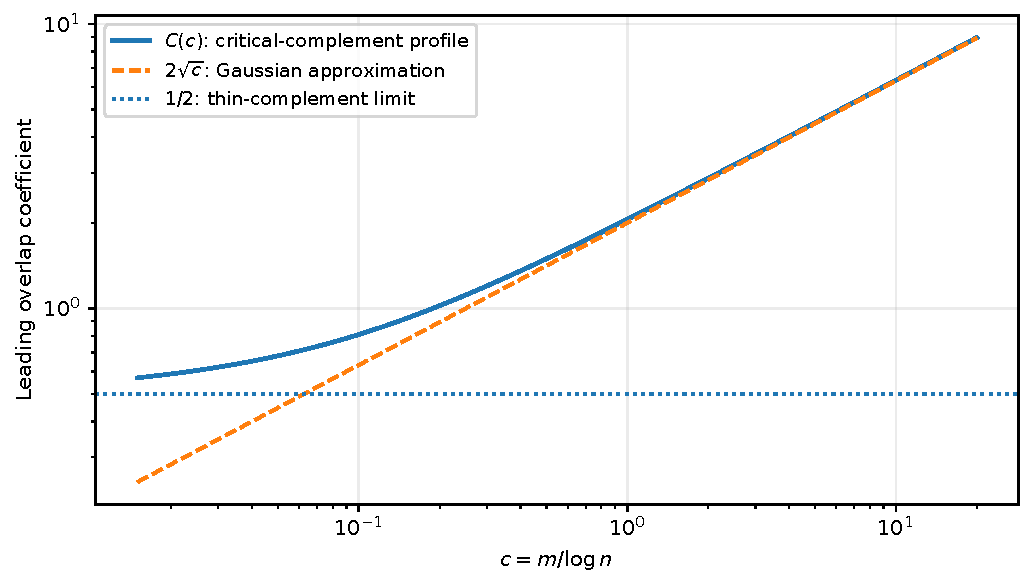
\includegraphics[width=.94\linewidth]{figures/crossover.pdf}
\caption{The critical coefficient $C(c)$ in \eqref{eq:critical}. The
Gaussian expression $2\sqrt c$ is its large-$c$ limit, not its value
throughout the critical window. The constant $1/2$ is the thin-complement
limit. The curves are deterministic evaluations of the theorem's
Lambert-$W$ formula, not Monte Carlo estimates.}
\label{fig:crossover}
\end{figure}

\section{Entropy for growing complements and the information gap}
\label{sec:entropy}

\subsection{A density and entropy limit for the complement}
Define the standardized density
\begin{equation}\label{eq:bstandard}
b_m(z)=\sqrt m\,g_m(m+\sqrt m\,z),
\end{equation}
extended by zero when its argument is nonpositive. From
\eqref{eq:saddle}, $\HH(0)=1$, and Taylor's formula for $I$,
\begin{equation}\label{eq:normaldensity}
b_m(z)\longrightarrow\phi(z)=(2\pi)^{-1/2}e^{-z^2/2}
\end{equation}
locally uniformly on $\R$.

\begin{lemma}[Uniform entropy integrability]\label{lem:entui}
There are $C,c>0$ such that, for all sufficiently large $m$ and all $z$,
\begin{equation}\label{eq:benvelope}
b_m(z)\le Ce^{-c|z|},\qquad
|b_m(z)\log b_m(z)|\le Ce^{-c|z|/2}.
\end{equation}
Consequently,
\begin{equation}\label{eq:complemententropy}
h_m=\frac12\log(2\pi e m)+o(1).
\end{equation}
\end{lemma}
\begin{proof}
The signed Gamma representation \eqref{eq:gammacomplement} and its
bounded total variation give $\sup_z b_m(z)\le C$. Log-concavity of
$g_m$ gives log-concavity of $b_m$. By \eqref{eq:normaldensity}, the
ratios $b_m(2)/b_m(0)$ and $b_m(-2)/b_m(0)$ are bounded strictly below
one for large $m$. Concavity of $\log b_m$ then bounds its secant slopes
outside $[-2,2]$ away from zero in the inward direction. Extrapolating
these slopes proves the first inequality in \eqref{eq:benvelope}; the
global bound handles the central interval. Zeros of the density cause
no problem, since the asserted upper bound is then automatic.

For $0<x\le1$, $x|\log x|\le C\sqrt x$. For $1\le x\le C$, the
function $x\log x$ is bounded; the exponential envelope restricts this
case to a bounded interval. This proves the second inequality.
Dominated convergence in \eqref{eq:normaldensity} gives
\[
-\int b_m\log b_m\longrightarrow-\int\phi\log\phi
 =\frac12\log(2\pi e).
\]
The entropy change under scaling by $\sqrt m$ is $\tfrac12\log m$,
proving \eqref{eq:complemententropy}.
\end{proof}

\subsection{Entropy after conditioning}
\begin{proof}[Proof of \eqref{eq:growingkl}]
Under the density $p^*_{n,m}$ in \eqref{eq:udensity}, change variables
$u=m+\sqrt m\,z$. The resulting density is
\begin{equation}\label{eq:conditionedstandard}
b_m(z)\,\frac{f_{n,m}(r_m-m-\sqrt m\,z)}{a_n}.
\end{equation}
The ratio in \eqref{eq:conditionedstandard} is uniformly bounded by
\eqref{eq:globalf} and $a_n\asymp\eps_n$. On any fixed compact interval
of $z$, it tends uniformly to one, because $r_m-m=O(1)$ and
$\sqrt m=o(\sqrt n)$. Split
\[
\log g_m(m+\sqrt m\,z)=-\frac12\log m+\log b_m(z).
\]
The first term integrates exactly to $-\tfrac12\log m$ since
\eqref{eq:conditionedstandard} is a probability density. This exact
normalization avoids multiplying an uncontrolled convergence error by
$\log m$. For the second term, Lemma~\ref{lem:entui} and the bounded
ratio permit dominated convergence. Therefore
\[
\int p^*_{n,m}\log g_m
 =-\frac12\log m+\int\phi\log\phi+o(1)
 =-\frac12\log(2\pi e m)+o(1).
\]
Finally $-\log a_n=\tfrac12\log(2\pi n)+o(1)$.
Substitution into \eqref{eq:entropyexact} proves
$D_{n,m}=\tfrac12\log(n/m)-\tfrac12+o(1)$.
\end{proof}

\subsection{Full-configuration entropy and a channel identity}
\begin{proof}[Proof of \eqref{eq:fullkl} and \eqref{eq:infogap}]
Let $G_n=\mu_n-T_n\ge0$ under $P_n$, and write $F_n$ for the centered
density of $T_n-\mu_n$ under $Q_n$. Convolving the prefix density for
$m=0$ with the bounded complement shows
\[
\sup_vF_n(v)\le C\eps_n,\qquad
F_n(v)/\eps_n\longrightarrow1
\]
uniformly on fixed compact intervals. The slack density under $P_n$ is
\[
\frac{e^{-g}F_n(-g)}{a_n}\ind_{\{g\ge0\}}.
\]
It converges pointwise to $e^{-g}$ and is bounded by $Ce^{-g}$.
Dominated convergence with weight $1+g$ gives $\E_{P_n}G_n\to1$.
The full likelihood yields the exact entropy identity
\[
\KL(P_n\Vert Q_n)=-\log a_n-\E_{P_n}G_n,
\]
proving \eqref{eq:fullkl}.

Subtract the fixed-complement formula \eqref{eq:fixedkl}; the limit is
$h_m-1$. Since $Z_m=R_m+E$ with $E$ independent, the standard entropy
identity for this additive channel is
\[
I(R_m;Z_m)=h(Z_m)-h(Z_m\mid R_m)=h_m-h(E)=h_m-1.
\]
All quantities are finite by Proposition~\ref{prop:profile}; equivalently,
the identity follows directly by integrating the log ratio of the
conditional density $e^{-(z-r)}\ind_{z\ge r}$ and $g_m(z)$.
It is nonnegative by relative entropy. It is strictly positive here:
zero mutual information would make $R_m$ and $R_m+E$ independent, whereas
$\Cov(R_m,R_m+E)=\Var(R_m)>0$. This completes
Theorem~\ref{thm:entropy}.
\end{proof}

\section{Phase structure, endpoint scales, and examples}
\label{sec:interpretation}

\subsection{Which constants remember the phase?}
\begin{proposition}[Phase identities]\label{prop:phase}
For fixed $m$, $K_{q,\rho,m}$ and $h_m$ are continuous in $\rho>0$.
The overlap constant satisfies
\begin{equation}\label{eq:Kderivative}
\rho\frac{\partial K_{q,\rho,m}}{\partial\rho}=r_m>0.
\end{equation}
At the phase boundary, with parameters extended continuously,
\begin{equation}\label{eq:phaseglue}
R_m\big|_{\rho=q^{-1}}\ \overset{d}=\
R_{m+1}\big|_{\rho=1},
\end{equation}
and the corresponding $K$ and $h$ constants agree. At fixed $q,\rho$,
$h_{m+1}>h_m$ and
\begin{equation}\label{eq:Krec}
K_{m+1}-K_m=\log\frac{\rho q^{-(m+1)}}
                                  {1-e^{-\rho q^{-(m+1)}}}.
\end{equation}
\end{proposition}
\begin{proof}
The series for $K_m$ and its derivative converge locally uniformly in
$\rho$, using the small-cap expansion in the tail. Differentiating
one term with cap $a$ gives
\[
a\frac\dd{\dd a}\log\frac a{1-e^{-a}}
 =1-\frac a{e^a-1}=b(a).
\]
Summing yields \eqref{eq:Kderivative}. Continuity of $h_m$ follows from
\eqref{eq:gprofile} and dominated convergence: on compact $\rho$-ranges
the supports $A_m$ and amplitudes $e^{K_m}$ are bounded, the entropy
integrand on a fixed compact interval is bounded, and the remaining
tail has a common exponential envelope. The CDF $F_q$ is continuous.

Reindexing the caps gives \eqref{eq:phaseglue} and \eqref{eq:Krec}.
For entropy monotonicity, $Z_{m+1}$ is the sum of $Z_m$ and an independent
nondegenerate truncated exponential $Y_{-(m+1)}$. Therefore
\[
h_{m+1}-h_m=I\bigl(Y_{-(m+1)};Z_m+Y_{-(m+1)}\bigr)>0.
\]
Strict positivity follows as before from a nonzero covariance and finite
second moments.
\end{proof}
The phase identity also checks the indexing convention. The same tilt
written with $\rho=q^{-1}$ and bulk index $n$ is written with $\rho=1$
and index $n+1$. To observe the same prefix one must replace $m$ by
$m+1$. The constants then match, while replacing $n$ by $n+1$ changes
the fixed-complement expansions only at smaller orders.

The leading crossover \eqref{eq:unified} forgets $q$ and $\rho$.
The fixed-complement constant does not: \eqref{eq:Kderivative} proves
strict phase dependence of the overlap correction, not merely a numerical
suggestion. We have not proved monotonicity of $h_m$ in $\rho$; its
continuity and exact formula suffice for the results here.

\subsection{Returning to the original small threshold}
Let $L_n=\log(1/x_n)$ and $a=\log(1/q)$. Equation~\eqref{eq:meanvar}
gives
\begin{equation}\label{eq:endpointscale}
x_n\sim\frac{nq^{n+1}}\rho,\qquad
L_n=an-\log n+O(1),\qquad
n=\frac{L_n+\log L_n}{a}+O(1).
\end{equation}
Consequently the crossover $m\asymp\log n$ occurs at
\begin{equation}\label{eq:doublylog}
m\asymp\log\log(1/x_n)
\end{equation}
in the original endpoint parameter. This scale is much smaller than
the effective dimension, which is of order $\log(1/x_n)$.
For fixed $m$, the two leading endpoint formulas become
\begin{align}
\ov_{n,m}
 &=\sqrt{\frac{a}{2\pi L_n}}
   \left[\frac12\log L_n+\frac12\log\frac{2\pi}{a}+1+K_m\right]
     +o(L_n^{-1/2}),\label{eq:endpointtv}\\
D_{n,m}&=\frac12\log L_n+\frac12\log\frac{2\pi}{a}-h_m+o(1).
\label{eq:endpointkl}
\end{align}
These statements are along the fixed-phase sequence in
\eqref{eq:tilt}. They do not suppress the phase by replacing it with
an averaged constant.

\subsection{Four illustrative complement scales}
For $m=0$, the observer sees every bulk coordinate but not the infinite
boundary tail. Equations~\eqref{eq:fixedtv} and \eqref{eq:fixedkl} give
$\ov\asymp\log n/\sqrt n$ and $D\sim\tfrac12\log n$. The finite entropy
loss relative to seeing everything is $h_0-1$.

For $m\sim\log n$, the overlap is
$C(1)\log n/\sqrt{2\pi n}$, where numerical evaluation gives
$C(1)\approx2.055967111$. Using the Gaussian value $2$ would miss a
nonvanishing proportion of the leading coefficient. Entropy is already
$\tfrac12\log(n/\log n)-\tfrac12+o(1)$.

For $m\sim n^\alpha$, $0<\alpha<1$,
\begin{align*}
\ov_{n,m}&\sim\sqrt{\frac{2(1-\alpha)}\pi}\,
             n^{(\alpha-1)/2}\sqrt{\log n},\\
D_{n,m}&=\frac{1-\alpha}{2}\log n-\frac12+o(1).
\end{align*}
For $m\sim n/(\log n)^\beta$, $\beta>0$,
\begin{align*}
\ov_{n,m}&\sim\sqrt{\frac{2\beta}\pi}\,
            (\log n)^{-\beta/2}\sqrt{\log\log n},\\
D_{n,m}&=\frac\beta2\log\log n-\frac12+o(1).
\end{align*}
The final example makes the distinction between the two divergence
parameters especially clear: the total-variation overlap is small but
entropy may diverge only at a doubly logarithmic rate.

\subsection{A warning about nonuniform fixed-complement formulas}
For growing $m$, \eqref{eq:Krec} gives
\begin{equation}\label{eq:Kgrowth}
K_m=\frac{\log(1/q)}2m(m+1)+m\log\rho+O(1).
\end{equation}
Meanwhile $A_m$ grows geometrically in $m$. Thus the fixed-$m$ tail
crossing condition $\log(e^{K_m}/\eps_n)>A_m$ can fail badly for a
moving $m$. Substituting \eqref{eq:Kgrowth} into \eqref{eq:fixedtv} is
not legitimate. For example, if $m$ is of order $\sqrt{\log n}$, the
putative $K_m$ correction is of order $\log n$, yet
Theorem~\ref{thm:crossover} still gives the thin-complement coefficient
$1/2$. The profile has not reached its eventual pure exponential tail
at the likelihood level being tested. This is exactly the sort of
nonuniformity that the crossover theorem resolves.

\section{Reproducible numerical diagnostics}
\label{sec:numerics}

\subsection{What is computed}
The accompanying Python code computes the boundary density through
\eqref{eq:gprofile}, using Fourier inversion of the \emph{unconditioned}
geometric uniform CDF. It then evaluates the exact one-dimensional
likelihood formulas of Proposition~\ref{prop:likelihood}. The prefix
density is obtained by the signed Gamma formula
\eqref{eq:prefixgamma}. This is a direct calculation for the geometric
model, not a finite-simplex proxy and not a Monte Carlo experiment.

There are still numerical approximations. The CDF is evaluated on a
finite Fourier grid with a geometrically truncated product, followed
by cubic interpolation. Prefix caps at least $64$ are replaced by
unbounded exponentials. For the dyadic $\rho=1$ case the sum of the
omitted truncation probabilities is about $1.604\times10^{-28}$.
This is an unconditional coupling bound; it is not, by itself, an
interval-certified bound for every conditional entropy integral.
Adaptive quadrature and floating-point evaluation introduce further
errors. None of these computations is used in the proofs.

\subsection{Boundary constants}
Table~\ref{tab:boundary} gives representative dyadic constants. The
entropy gap is $h_m-1$, in natural-logarithm units. The $m=0$ row at
$\rho=1$ has
\[
K_0\approx0.944809318,\qquad h_0\approx1.265596223,
\qquad \mathscr E_0\approx0.632308464.
\]
For the same phase, $\delta\approx-0.9428328015$. These values are
computed independently from the formulas for the variance constant,
boundary profile, and covariance coefficient; the coefficient is not
fitted from the finite-$n$ table.

\begin{table}[ht]
\centering\small
\begin{tabular}{@{}rr rrr@{}}
\toprule
$\rho$ & $m$ & $K_m$ & $h_m$ & $I(R_m;R_m+E)$\\
\midrule
\inputtable{data/boundary_table.tex}
\bottomrule
\end{tabular}
\caption{Floating-point boundary constants for $q=1/2$.
The infinite boundary tail is included in every row.}
\label{tab:boundary}
\end{table}

\subsection{Finite-size tests of the constants}
In Table~\ref{tab:finite}, define
\[
R^{\rm TV}_n=\frac{\ov_{n,0}}{\eps_n}
             -\log(1/\eps_n)-1-K_0,
\qquad
R^{\rm KL}_n=D_{n,0}-\log(1/\eps_n)+h_0.
\]
Theorems predict $R^{\rm TV}_n\to0$ and
$nR^{\rm KL}_n\to\mathscr E_0\approx0.632308464$.
The negative overlap residual is mostly $-\Delta_0(\eps_n)$, as
shown in Figure~\ref{fig:deficit}.

\begin{table}[ht]
\centering\small
\begin{tabular}{@{}r rrrr@{}}
\toprule
$n$ & $\ov_{n,0}$ & $R^{\rm TV}_n$ & $D_{n,0}$ & $nR^{\rm KL}_n$\\
\midrule
\inputtable{data/finite_table.tex}
\bottomrule
\end{tabular}
\caption{Direct geometric-model diagnostics for $q=1/2$, $\rho=1$, $m=0$.
Theorem~\ref{thm:fixed} concerns the limits, not an assertion that the
two-term overlap expansion is already highly accurate at these sizes.}
\label{tab:finite}
\end{table}

\begin{figure}[ht]
\centering
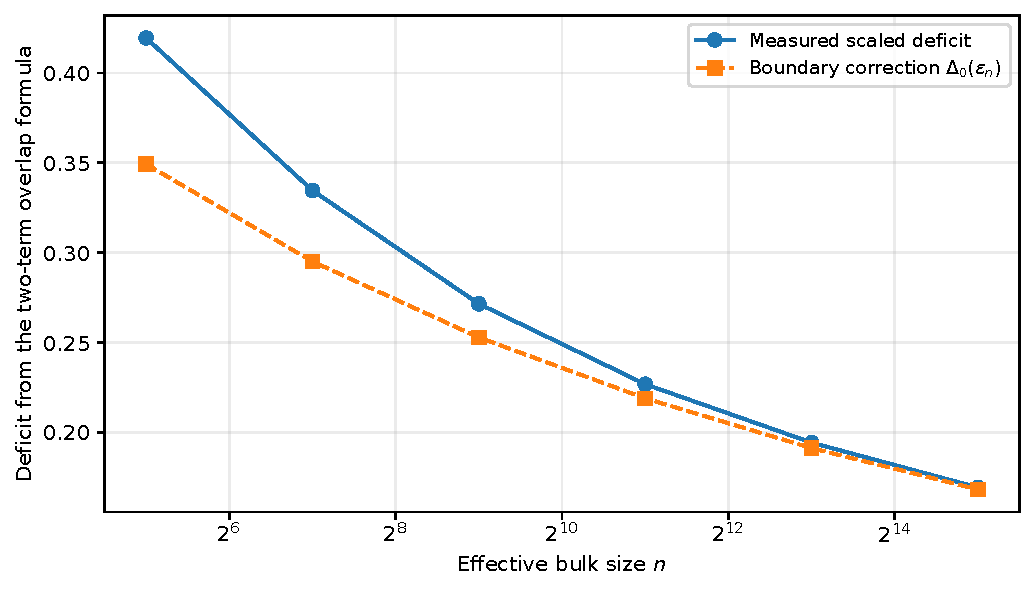
\includegraphics[width=.94\linewidth]{figures/boundary_deficit.pdf}
\caption{The measured scaled overlap deficit and the independently
computed compact correction $\Delta_0(\eps_n)$. Their difference is
consistent with the $O((\log n)^3/n)$ error in
\eqref{eq:correctedtv}. This plot diagnoses a slow boundary effect;
it is not a proof of the asymptotic bound.}
\label{fig:deficit}
\end{figure}

\subsection{Recorded checks and reproduction}
The delivered run used Python 3.13.5, NumPy 2.3.5, and SciPy 1.17.0.
Across the twelve boundary computations, increasing the Fourier grid
from $2^{15}$ to $2^{16}$ points changed the computed entropy by at most
$1.27\times10^{-14}$, and the largest mass discrepancy was
$6.44\times10^{-15}$. The residuals in the Lambert-$W$ rate identity
were at most $2.23\times10^{-16}$. These small discrepancies are
internal consistency checks, not certified error bars.

The quadrature explicitly separates the compact boundary from the
exponential tail. In particular, it does not ask a generic adaptive
integrator to find a short exponential boundary layer inside an
interval whose length is of order $n$. The remaining profile-tail mass
in the principal dyadic calculations is bounded by $e^{-82}$ before
its use in the conditional formulas.

\noindent\begin{minipage}{\linewidth}
From the package directory, the computations and article can be rebuilt
with
\begin{verbatim}
python code/verify.py
python code/make_figures.py
latexmk -pdf -interaction=nonstopmode -halt-on-error article.tex
\end{verbatim}
\end{minipage}

The pre-generated figures and table fragments are included. Rebuilding
only the PDF requires no Python execution and no network access. The
JSON receipt records the numerical environment, check results, and their
scope. Platform and library changes may alter the last displayed digits.

\section{Further research questions and topics}
\label{sec:questions}

The geometric-prefix critical-complement problem is resolved by the
three main theorems. The following questions are not presented as solved.
Some extend the same explicit repository frontier to settings where the
proof mechanisms no longer transfer automatically.

\begin{question}[Arbitrary observation masks]
For general subsets of geometric coordinates, can the crossover be
classified by a complement cumulant function rather than the number
$m$? A mask may hide isolated large-cap coordinates, a boundary cluster,
or both. A variance fraction suffices for the qualitative endpoint,
but the present theorem shows that the limiting variance fraction alone
does not determine
sharp overlap rates in a singular regime. An appropriate replacement
for the Gamma rate function should depend on the hidden cap profile.
\end{question}

\begin{question}[General summable weights]
Which positive summable weight sequences admit an analogue of the
signed correction with bounded exponential variation? For polynomial
weights, the boundary layer has a growing number of coordinates and
need not be an $O(1)$ correction to a Gamma law. Prove a sharp
critical-complement theorem in at least one such nongeometric class,
and identify whether the logarithmic crossover scale survives.
\end{question}

\begin{question}[Second-order crossover terms]
In the window $m\sim c\log n$, the first neglected terms in
\eqref{eq:level} contain $\log\HH(1-1/y)$, integer rounding of $m$, and
the difference between $\log(n/m)$ and $\log n$. Derive the complete
next-order overlap expansion, uniformly for $c$ in compact subsets of
$(0,\infty)$, and exhibit the reappearance of the geometric phase.
The leading theorem gives the correct starting points for both
likelihood crossings.
\end{question}

\begin{question}[A sharp asymptotic for the compact deficit]
Determine the asymptotics of $\Delta_m(a)$ as $a\downarrow0$ from the
small-argument Fabius expansion, including phase oscillations and an
explicit error bound. Equation~\eqref{eq:Jexact} reduces the slow
fixed-complement correction to a concrete one-dimensional inverse-level
problem. This would turn \eqref{eq:correctedtv} into a fully expanded
endpoint transseries rather than a formula retaining one exact integral.
\end{question}

\begin{question}[A moving geometric ratio]
Let $q=q_n\uparrow1$. The uniform exponential-variation constants in
Lemma~\ref{lem:signed} may then diverge and the boundary tail ceases
to be a fixed-size perturbation. Find the joint scaling of $1-q_n$,
$n$, and $m$ that separates Gamma-type, boundary-dominated, and
intermediate limits. The fixed-$q$ theorem should not be used as a
uniform assertion in this regime.
\end{question}

\begin{question}[Other endpoint densities]
Replace the uniform coordinates by densities behaving like
$c_jx^{\alpha_j-1}$ near zero. Exponential tilting suggests Gamma
coordinates with varying shapes. Under what quantitative regularity
hypotheses does an explicit complement rate function yield a version
of \eqref{eq:unified}? Even the constant-shape case requires tracking
which boundary correction is genuinely bounded and which alters the
large-deviation exponent.
\end{question}

\begin{question}[Several simultaneous constraints]
For two or more weighted sums constrained to a small orthant, the
likelihood becomes a multivariate boundary convolution. Determine the
analogue of $I(R_m;R_m+E)$ and classify the overlap by the volume of a
multivariate density level set. The geometry of that level set, not
just a determinant of a covariance matrix, should matter at critical
complement sizes.
\end{question}

\begin{question}[Equality, windows, and inequality conditioning]
Give a unified theorem when $T_n$ is conditioned on an interval of
width $w_n$ immediately below $\mu_n$, allowing $w_n\to0$, $w_n\to w$,
and $w_n\to\infty$. The exponential slack in this paper should be
replaced by a truncated kernel or by exact-level conditioning in the
appropriate limits. Determine precisely when the leading logarithmic
overlap mechanism changes.
\end{question}

\begin{question}[Phase entropy and comparison inequalities]
The phase derivative of $K_m$ is explicit, but the derivative and
possible monotonicity of $h_m$ in $\rho$ have not been settled here.
Find useful analytic bounds on $h_m-1$ and on the covariance in
\eqref{eq:Ecoeff}, uniformly over a phase cell. Such bounds would
control information loss without numerical Fourier inversion.
\end{question}

\begin{question}[Certified computation and formalization]
Construct an interval-certified evaluator for $g_m$, $h_m$,
$\Delta_m$, and $\mathscr E_m$, and formalize the likelihood and signed
Gamma identities in Lean. A complete formalization should separate
measure-theoretic conditioning from the asymptotic density estimates,
and should prove uniform tail bounds rather than importing numerical
plots as certificates. Quantitative constants suitable for verified
finite-$n$ bounds remain a practical target.
\end{question}

\section{Proof status and a formalization roadmap}
\label{sec:status}

The article provides conventional proofs of
Theorems~\ref{thm:fixed}, \ref{thm:crossover}, and \ref{thm:entropy},
including the displayed hypotheses, constants, and remainders. The
principal imported analytic fact is convolution preservation of
log-concavity. The remaining density estimates are derived from the
exact signed convolution and Stirling's formula. We do not invoke an
unspecified local limit theorem with an unverified uniformity range.

For integration into the repository, a sensible dependency order is:
first the countable product tilt and exact likelihood; then the
truncated-exponential/signed-Gamma identity and its weighted variation
bounds; then central density estimates and the complement saddle
estimate; finally the overlap and entropy limits. The finite algebra
and the countable measure-theoretic interface are logically independent
of the analytic large-$n$ step. This separation should make auditing
and alternative proofs easier.

No new Lean or Rocq proof file is included, and no repository-wide build
or axiom audit was run. The included Python programs test numerical
consequences; they do not certify the theorems. The prior research
manuscripts are themselves distinguished from the repository's formally
proved Fabius development. None of those statuses is upgraded merely
because this paper builds on the same topic.

The resolved scope is exact: fixed geometric ratio, a fixed tilt phase,
inequality conditioning at the tilted mean, and an observed prefix
whose missing bulk size is sublinear. Within that scope the qualitative
singular endpoint has been replaced by explicit laws. Beyond it,
Section~\ref{sec:questions} records the remaining problems rather than
silently extrapolating the results.

\appendix
\section{Numerical identities used by the implementation}
\label{app:numerics}

\subsection{Finite signed inclusion--exclusion}
For a finite collection of caps $a_1,\ldots,a_k$, the density of the sum
of independent $p_{a_j}$ variables is exactly
\begin{equation}\label{eq:inclusion}
\frac1{\prod_{j=1}^k(1-e^{-a_j})}
\sum_{J\subseteq\{1,\ldots,k\}}(-1)^{|J|}e^{-a_J}
                  \gamma_k(s-a_J),\qquad
 a_J=\sum_{j\in J}a_j.
\end{equation}
This follows by expanding the product of signed measures in
\eqref{eq:prefixgamma}. The implementation retains only the caps below
a chosen numerical threshold. The remaining variables are full
exponentials, but still contribute to the Gamma shape $k$. Thus the
number of signed terms depends on the number of moderate caps, not
on the effective dimension $n$.

A variable with law $p_a$ is an exponential conditioned to be at most
$a$. It can be coupled with an unconditioned exponential with mismatch
probability $e^{-a}$. A union bound gives the recorded omission bound
$\sum e^{-a_j}$ for the replaced coordinates. Formula~\eqref{eq:inclusion}
is exact before this computational simplification.

\subsection{Fourier inversion of the boundary CDF}
Let $V=\sum_{\ell\ge0}cq^\ell U_\ell$ have support
$[0,A]$, $A=c/(1-q)$. Its Fourier transform under the convention
$\widehat f(\omega)=\E e^{-i\omega V}$ is
\begin{equation}\label{eq:fourier}
\widehat f(\omega)
 =e^{-i\omega A/2}\prod_{\ell\ge0}
       \operatorname{sinc}\!\left(\frac{\omega cq^\ell}{2}\right),
\qquad \operatorname{sinc}(z)=\frac{\sin z}{z}.
\end{equation}
The removable value at zero is one. The code uses a periodic interval
of length $2A$, which contains the support without an interior wrap,
and integrates its Fourier series by dividing each nonzero coefficient
by $i\omega$. The zero-frequency term contributes $u/(2A)$.
Subtracting the primitive's value at zero produces the CDF. The density
$g_m$ is then recovered by multiplying the CDF by $e^{K_m-u}$.

Finite Fourier truncation, truncation of the infinite product, and
interpolation mean that the implemented CDF is not an exact real
function. Increasing the grid supplies a convergence check; it is not
an interval proof. The tail identities used after $u=A_m$ are analytic,
so no Fourier evaluation is needed there. In particular,
\begin{align*}
\int_{A_m}^\infty g_m(u)\,\dd u&=e^{K_m-A_m},\\
-\int_{A_m}^\infty g_m(u)\log g_m(u)\,\dd u
 &=e^{K_m-A_m}(A_m+1-K_m).
\end{align*}
These formulas improve both stability and reproducibility.

\section{Elementary checks on the crossover roots}
\label{app:roots}

The derivative $I'(y)=1-1/y$ is negative on $(0,1)$ and positive on
$(1,\infty)$. Since $I(1)=0$ and $I$ tends to infinity at both ends,
there are exactly two roots for every positive level. The equation
$I(y)=z$ is equivalent to $(-y)e^{-y}=-e^{-1-z}$, proving
\eqref{eq:roots}.

For $z\downarrow0$, write $y=1+v$ and expand
$I(1+v)=v^2/2-v^3/3+O(v^4)$. Thus
\[
y_\pm(z)=1\pm\sqrt{2z}+O(z),\qquad
 y_+(z)-y_-(z)\sim2\sqrt{2z}.
\]
For $z\to\infty$, the lower root tends to zero and satisfies
$y_-=e^{-1-z+y_-}\sim e^{-1-z}$. The upper root satisfies
$y_+=z+1+\log y_+$, hence $y_+/z\to1$. These observations justify all
endpoint limits used in Section~\ref{sec:crossover}.

They also show that the leading equivalent remains positive and tends
to zero for every $m=o(n)$: on the Gaussian side it is controlled by
$\sqrt{(m/n)\log(n/m)}$, and on the other two sides it is of order
$\log n/\sqrt n$. The crossover formula is therefore compatible with
the predecessor's qualitative conclusion $\TV\to1$, while supplying
information that that conclusion alone does not contain.

\clearpage
\begin{thebibliography}{9}

\bibitem{repo-uniform}
\repo\ research manuscript collection, repository maintained by
V.~Reshetnikov,
\emph{Sharp Conditioning Laws for Uniform Random Series:
Variance thresholds, boundary phases, Brownian bridges, and rare-event sampling}.
Research manuscript dated 28 September 2026; README and article inspected
in the 30 September snapshot \snap.
\newblock Repository path:
\path{Analysis/FabiusFunction/docs/semi-formalized-research-frontiers/drafts/representations/Sharp_Conditioning_Laws_Uniform_Random_Series/}.
\newblock\url{https://github.com/VladimirReshetnikov/ProveIt/tree/0a543d5e435df885f78ca731d71856f3ee0ab2d4/Analysis/FabiusFunction/docs/semi-formalized-research-frontiers/drafts/representations/Sharp_Conditioning_Laws_Uniform_Random_Series}.
This is an unformalized repository research manuscript, cited for the
prior claims and the explicitly remaining critical-complement question,
not treated as a refereed publication.

\bibitem{repo-lacunary}
\repo\ research manuscript collection, repository maintained by
V.~Reshetnikov,
\emph{Sharp Conditioning Laws for Fabius and Lacunary Random Series}.
Research manuscript dated 28 September 2026; README and contribution
summary inspected in the same snapshot.
\newblock Repository path:
\path{Analysis/FabiusFunction/docs/semi-formalized-research-frontiers/drafts/representations/Sharp_Conditioning_Laws_Fabius_Lacunary_Series/}.
\newblock\url{https://github.com/VladimirReshetnikov/ProveIt/tree/0a543d5e435df885f78ca731d71856f3ee0ab2d4/Analysis/FabiusFunction/docs/semi-formalized-research-frontiers/drafts/representations/Sharp_Conditioning_Laws_Fabius_Lacunary_Series}.
No formal status is inferred from the repository location.

\bibitem{df}
P.~Diaconis and D.~Freedman,
\emph{Conditional limit theorems for exponential families and finite
versions of de Finetti's theorem}.
Journal of Theoretical Probability \textbf{1} (1988), no.~4, 381--410.
\newblock Berkeley technical-report record:
\url{https://digicoll.lib.berkeley.edu/record/86140}.
Cited for the classical conditional-limit context; the present proofs
do not invoke a theorem from this paper.

\bibitem{dz}
A.~Dembo and O.~Zeitouni,
\emph{Refinements of the Gibbs conditioning principle}.
Probability Theory and Related Fields \textbf{104} (1996), 1--14.
\newblock\url{https://doi.org/10.1007/BF01303799}.
Cited for the classical growing-block context, not as a uniform
critical-complement estimate being assumed here.

\bibitem{arias}
J.~Arias de Reyna,
\emph{An infinitely differentiable function with compact support:
Definition and properties}.
English version, arXiv:1702.05442 (2017), of the 1982 paper in
Revista de la Real Academia de Ciencias Exactas, F\'isicas y Naturales
de Madrid \textbf{76}, 21--38.
\newblock\url{https://arxiv.org/abs/1702.05442}.

\bibitem{prekopa}
A.~Pr\'ekopa,
\emph{On logarithmic concave measures and functions}.
Acta Scientiarum Mathematicarum (Szeged) \textbf{34} (1973), 335--343.
\newblock Theorem~7 supplies convolution preservation of log-concavity.
Author-hosted paper:
\url{https://rutcor.rutgers.edu/~prekopa/SCIENT2.pdf}.

\end{thebibliography}
\end{document}
